\documentclass{a4beamer}
%% Lectures - common definitions

\usextensions{tikz}
\usetikzlibrary{shapes.multipart,shapes.callouts,shapes.geometric}
\input{fix-callouts.inc} % Fixes absolute positioning of rectangle callouts

\newif\ifbigpages \bigpagesfalse
\ifdim\paperwidth >20cm
	\bigpagestrue
\fi

\tikzset{%
	note/.style={rectangle callout,draw=none,callout pointer width=1em,%
		align=flush left,font=\footnotesize,inner sep=0.5em,%
		fill=blue!15,fill opacity=0.95,text opacity=1.0,callout absolute pointer=#1},
	node distance=2em and 2.75em
}
\ifbigpages
	% Scale all arrow tips by the factor of 2.5
	\let\old@pgf@arrow@call=\pgf@arrow@call
	\def\pgf@arrow@call#1{%
		\@tempdima=\pgflinewidth%
		\pgfsetlinewidth{2.5\pgflinewidth}%
		\old@pgf@arrow@call{#1}%
		\pgfsetlinewidth{\@tempdima}%
	}
	\def\pgfarrowsleftextend#1{\pgfmathsetlength{\pgf@xa}{1.5*#1}}
	\def\pgfarrowsrightextend#1{\pgfmathsetlength{\pgf@xb}{1.5*#1}}
\fi

%% Load listings package
\usepackage{listings}

%% Are we inside a comment?
\newif\iflstcomment \lstcommentfalse

\lstset{%
	tabsize=4,
	showstringspaces=false,
	basicstyle=\linespread{1.25}\ttfamily\small,
	keywordstyle=\bfseries,
	commentstyle=\lstcommentstyle,
	numbers=left,
	numberstyle=\footnotesize\color{gray},
	xleftmargin=2.5em,
	extendedchars=true,
	escapechar=\$,
	escapebegin=\iflstcomment\begingroup\lstcommentstyle\fi,
	escapeend=\iflstcomment\endgroup\fi
}

\def\lstcommentstyle{\color{gray}}

\lst@AddToHook{AfterBeginComment}{\global\lstcommenttrue}
\let\orig@lst@EndComment=\lst@EndComment
\def\lst@EndComment{\global\lstcommentfalse\orig@lst@EndComment}
\lst@AddToHookAtTop{EOL}{%
	\lst@ifLmode\global\lstcommentfalse\fi% XXX Sloppy way to determine comment end
}

%% Python with docstrings treated as comments
\lstdefinelanguage[doc]{python}[]{python}{%
	deletestring=[s]{"""}{"""},%
	morecomment=[s]{"""}{"""}%
}%

%% JavaScript language
\lstdefinelanguage{javascript}%
	{morekeywords={break,case,catch,%
		const,constructor,continue,default,do,else,false,%
		finally,for,function,if,in,instanceof,%
		new,null,prototype,%
		return,switch,this,throw,%
		true,try,typeof,var,while},%
	sensitive,%
	morecomment=[l]//,%
	morecomment=[s]{/*}{*/},%
	morestring=[b]",%
	morestring=[b]',%
}[keywords,comments,strings]%

%% C# language (4.0?)
\lstdefinelanguage{csharp}%
	{morekeywords={abstract,as,%
		base,bool,byte,case,catch,char,%
		checked,class,const,continue,%
		decimal,default,delegate,do,double,%
		else,enum,event,explicit,extern,%
		false,finally,fixed,float,for,foreach,%
		goto,if,implicit,in,int,interface,%
		internal,is,lock,long,%
		namespace,new,null,object,operator,out,%
		override,params,private,protected,public,%
		readonly,ref,return,sbyte,sealed,%
		short,sizeof,stackalloc,static,string,%
		struct,switch,this,throw,true,try,%
		typeof,uint,ulong,unchecked,unsafe,ushort,%
		using,virtual,void,volatile,while%
	},%
	sensitive,%
	morecomment=[l]//,%
	morecomment=[s]{/*}{*/},%
	morestring=[b]",%
	morestring=[b]',%
}[keywords,comments,strings]%

%% Translation for fact environment
\deftranslation[to=russian]{Fact}{Наблюдение}

%% Inline code snippets
\def\code#1{\texttt{#1}}
\def\codekw#1{\code{\textbf{#1}}}

\def\quoteauthor#1{\par\footnotesize\upshape\hfill—~#1}

%% English term
\def\engterm#1{(англ. \textit{#1})}
%% Term with explanation below (to be used in diagrams)
\def\termwithexpl#1#2{#1\strut{}\\\small\color{gray}(\textit{#2})\strut{}}
%% External link
\def\extlink#1#2{\href{#1}{\color[rgb]{0.7,0.7,1.0}\dashbar{#2}}}
%% Internal link
\def\inlink#1#2{\hyperlink{#1}{\color[rgb]{0.7,0.7,1.0}\dashbar{#2}}}
%% Explanation for a list item
\def\itemexpl#1{\begingroup\small\vspace{0.75ex}#1\par\endgroup}



\usepackage{colortbl}

\def\ccell#1#2{\parbox{#1}{\centering #2 \\ \vspace{1.ex}}}
\def\colorcell#1{%
	{\hfill\color[rgb]{#1} \rule{0.15\textwidth}{2.5ex}\hfill}%
}


\lecturetitle{Программная инженерия. Лекция №1 — содержание ПИ.}
\title[Программная инженерия]{Программная инженерия: содержание дисциплины}
\author{Алексей Островский}
\institute{\small{Физико-технический учебно-научный центр НАН Украины}\vspace{2ex}}
\date{19 сентября 2014 г.}

\begin{document}
	\frame{\titlepage}
	
	\section{Вступление}
	
	\subsection{Определение программной инженерии}
	
	\frame{
		\frametitle{Определение программной инженерии}
		
		\begin{Definition}
			\textbf{Программная инженерия} (англ. \emph{software engineering}) — система методов, средств и~дисциплин планирования, 
			разработки, эксплуатации и~сопровождения программного обеспечения, готового к~внедрению.
		\end{Definition}
		
		\vspace{.5ex}
		\begin{Definition}[более полное]
			\textbf{Программная инженерия} — раздел компьютерных наук (англ. \emph{computer sciences}), 
			изучающий методы и средства построения компьютерных программ как продукта 
			теоретической и~инженерной деятельности разработчиков или их коллективов.
		\end{Definition}
		
		\vspace{1ex}
		\textbf{Основные критерии ПИ:} продуктивность, индустрия и качество.
	}
	
	\subsection{История ПИ}
	
	\frame{
		\frametitle{Предпосылки возникновения ПИ}
		
		Основная предпосылка появления программной инженерии: необходимость перехода 
		от~программирования \emph{как искусства} к~программированию \emph{как индустрии} в~связи с~усложнением программного обеспечения.
		
		\vspace{1.2ex}
		\begin{overlayarea}{\textwidth}{0.7\textheight}
			\begin{center}
				\only<1>{
					\textbf{Переход от единичного производства}

					\vspace{1ex}
					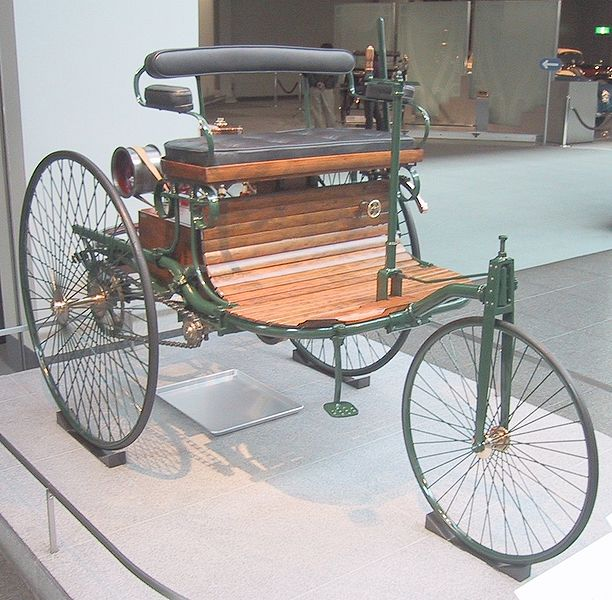
\includegraphics[height=0.5\textheight]{benz-car.jpg}

					\vspace{0.5ex}
					\figureexpl{Реконструкция автомобиля «Motorwagen» Карла Бенца, выпущенного в 1886 году.}
				}
				\only<2>{
					\textbf{\dots к массовому}

					\vspace{1ex}
					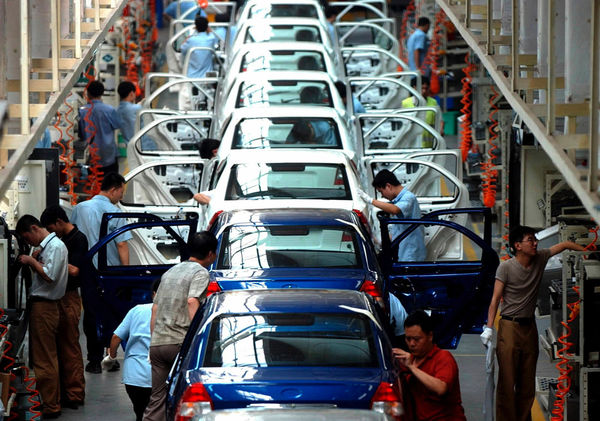
\includegraphics[height=0.5\textheight]{car-assembly-line.jpg}

					\vspace{0.5ex}
					\figureexpl{Современный конвеер для сборки автомобилей.}
				}
			\end{center}
		\end{overlayarea}
	}
	
	\frame{
		\frametitle{История возникновения ПИ}
		
		Первое упоминание программной инженерии — конференция НАТО 1968~г. в~связи с~кризисом программного обеспечения.
		
		\vspace{2ex}
		\begin{quote}
			Основная причина кризиса программного обеспечения — резкий рост мощностей вычислительных машин! 
			Проще говоря: нет вычислительной техники — нет~проблем с~разработкой программного обеспечения для~неё; 
			когда~же появилось несколько слабых компьютеров, появились первые проблемы, связанные с~разработкой программного обеспечения, 
			сейчас у~нас есть гигантские компьютеры, и~программирование стало столь~же гигантской проблемой.
			
			\vspace{0.5ex}
			\hfill\figureexpl{— Э. Дейкстра}
		\end{quote}
	}
	
	\frame{
		\frametitle{Программная инженерия в СССР}
		
		В СССР основы программной инженерии (технологии программирования) были заложены академиком 
		В.\,М. Глушковым в Институте кибернетики НАН УССР.
		
		\vspace{1ex}
		\begin{center}
			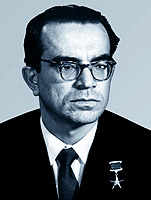
\includegraphics[height=0.4\textheight]{glushkov.jpg}

			\vspace{0.5ex}
			\figureexpl{Академик АН СССР и АН УССР Виктор Михайлович Глушков (1923—1982)}
		\end{center}
	}
	
	\section{Содержание ПИ}
	
	\subsection{Место ПИ среди компьютерных наук}
	
	\frame{
		\frametitle{Место ПИ среди компьютерных наук}
	
		Программная инженерия занимает центральное место среди компьютерных наук; 
		она задает парадигмы, теории и концепции для каждой из них, 
		определяет процессы разработки, применение, конфигурирование и развертывание созданного ПО.
	
		\begin{center}\tabcolsep=4pt\linespread{0.75}\small\extrarowheight=.1ex
			\begin{tabular}{|>{\vspace{.1ex}}p{0.25\textwidth}|*{3}{>{\vspace{.1ex}}p{0.2\textwidth}|}}
			\hline
				& \ccell{0.2\textwidth}{Теория, \\ концепции, \\ принципы} 
				& \ccell{0.2\textwidth}{Разработка} 
				& \ccell{0.2\textwidth}{Применение, \\ разворачивание, \\ конфигурирование} \\
			\hline
				\ccell{0.25\textwidth}{Информационные \\ системы} & & \colorcell{0.8,1.0,0.8} & \\ \hline
				\ccell{0.25\textwidth}{Информационные \\ технологии} & \colorcell{0.8,1.0,0.8} & \colorcell{0.5,1.0,0.5} & \colorcell{0.9,1.0,0.9} \\ \hline
				\ccell{0.25\textwidth}{Программная \\ инженерия} & \colorcell{0.2,1.0,0.2} & \colorcell{0.0,1.0,0.0} & \colorcell{0.2,1.0,0.2} \\ \hline
				\ccell{0.25\textwidth}{Системная \\ инженерия} & \colorcell{0.8,1.0,0.8} & \colorcell{0.4,1.0,0.4} & \colorcell{0.5,1.0,0.5} \\ \hline
				\ccell{0.25\textwidth}{Компьютерная \\ инженерия} & & \colorcell{0.9,1.0,0.9} & \colorcell{0.8,1.0,0.8} \\
			\hline
			\end{tabular}
		\end{center}
	}
	
	\frame{
		\frametitle{Теоретический фундамент ПИ}
		
		Программная инженерия основывается на математических дисциплинах:
		\begin{itemize}
			\item
			\textbf{теория алгоритмов} — нормальные алгоритмы, вычислимые функции, машина Тьюринга, граф-схемы, модели алгоритмов;
			\item
			\textbf{математическая логика} — формальный вывод утверждений;
			\item
			\textbf{теория управления} — принципы, методы и общие законы планирования и~управления в~сложных системах;
			\item
			\textbf{теория доказательств} — математическая теория вывода по~аксиомам и~утверждениям, теория верификации программ;
			\item
			\textbf{теория множеств} — формальное представление совокупностей объектов из~предметной области.
		\end{itemize}
	}
	
	\subsection{Составляющие ПИ}

	\frame{
		\frametitle{Составляющие ПИ}
		
		Программная инженерия состоит из двух частей — науки и инженерии программ:
		\begin{itemize}
			\item
			\textbf{теория разработки программ} — схемы, функции и композиции, теория верификации и~т.\,д.;
			\item
			\textbf{практика разработки программ} — применение практических методов программирования 
			и~соответствующих методов для описания, построения, верификации, тестирования и~оценки качества ПО.
		\end{itemize}
		
		Пересечение этих двух областей включает в~себя теорию и практику разработки сложных программных объектов.
	}
	
	\frame{
		\frametitle{Содержание дисциплины ПИ}
		
		Содержание дисциплины программной инженерии определено в стандарте SWEBOK 
		(\emph{software engineering body of knowledge}) — пять основных и~пять вспомогательных областей.
		
		\vspace{.5ex}
		Основные области программной инженерии:
		\begin{itemize}
			\item
			\textbf{инженерия требований} — выработка, анализ, спецификация и~корректировка требований к~программному обеспечению;
			\item
			\textbf{проектирование} — определение архитектуры ПО, компонентов, интерфейсов и~их~характеристик;
			\item
			\textbf{конструирование} — создание рабочего программного обеспечения;
			\item
			\textbf{тестирование} — проверка корректности выполнения ПО;
			\item
			\textbf{сопровождение} — поддержка ПО, минимизирующая затраты.
		\end{itemize}
	}
	
	\frame{
		\frametitle{Содержание дисциплины ПИ (продолжение)}
		
		Организационные области программной инженерии:
		\begin{itemize}
			\item
			\textbf{управление конфигурацией} — контроль над вносимыми в~ПО~изменениями с~целью обеспечить его~целостность;
			\item
			\textbf{управление проектом} — планирование и~координация процессов разработки и~сопровождения ПО;
			\item
			\textbf{процесс инженерии} — определение и~управление жизненным циклом программного обеспечения;
			\item
			\textbf{методы и инструменты инженерии} — компьютерные инструменты для~автоматизации процессов жизненного цикла~ПО;
			\item
			\textbf{инженерия качества} — измерение и~гарантирование качества программ.
		\end{itemize}
	}
	
	\section{Заключение}
	
	\subsection{Выводы}
	
	\frame{
		\frametitle{Выводы}
		
		\begin{enumerate}
			\item
			Программная инженерия — компьютерная наука, целью которой является применение принципов массового производства (т.\,е.~инженерии) \
			к~проектированию, разработке и~сопровождению программного обеспечения.
			
			\vspace{0.5ex}
			\item
			Основная причина развития программной инженерии — возрастающая сложность программных продуктов.

			\vspace{0.5ex}			
			\item
			Программная инженерия включает в~себя как~теоретические, так~и~прикладные аспекты. 
			Они предназначены для~определения жизненного цикла программного обеспечения и~решения возникающих в~процессе организационных вопросов.
		\end{enumerate}
	}

	\subsection{Материалы}
	
	\frame{
		\frametitle{Материалы}
		
		\begin{thebibliography}{9}
			\bibitem{1}
			Лаврищева Е.\,М.
			\newblock Учебники по программной инженерии.
			\newblock {\footnotesize (есть на \url{http://intuit.ru/})}
			\bibitem{2}
			Sommerville, Ian
			\newblock Software Engineering.
			\newblock {\footnotesize Pearson, 2011. — 790 p.}
			\newblock {\footnotesize (есть в Интернете)}
			\item
			\newblock Инструментально-технологический комплекс.
			\newblock {\footnotesize\url{http://sestudy.edu-ua.net/}}
		\end{thebibliography}
	}
	
	\frame{
		\frametitle{}
		
		\begin{center}
			\Huge Спасибо за внимание!
		\end{center}
	}
\end{document}
